\section{Bayesian modeling and inference for MJPs}
\label{sec:bayes_model}
%In practical situations, an MJP is noisily observed at
%a finite set of times. %with the observations themselves noisy. 
%This raises two questions: 
%%\begin{itemize}
%1) what is the underlying trajectory? and 2%)
%  what are the MJP parameters?
%%\end{itemize}
%  \vspace{-.1in}
%\textbf{Bayesian model:}
We first set up our Bayesian model of the data generation process. 
We model a latent piecewise-constant path $S(t)$ over $[0,t_{end})$ as an $N$-state MJP with rate matrix $A(\theta)$ and prior $\pi_0$ over $s_0 = S(0)$, the state at time $0$. 
We use both $\{S(t), t \in [0,t_{end})\}$ and $(s_0,S,T)$ (see section~\ref{sec:mjp}) to refer to the MJP path.
We place a prior $\prior(\theta)$ over the unknown $\theta$. 
For clarity we will assume $\pi_0$ is known (or we set it to a uniform distribution over the $N$ states). 
%In settings with multiple trajectories, we would place a Dirichlet prior over $\pi_0$. 
We have noisy measurements $X$ of the latent process, with likelihood $P(X|\{S(t),\ t \in [0,t_{end})\})$.
Again, for clarity we ignore any unknown parameters in the likelihood, else we can include them in $\theta$.
We assume the observation process has the following structure: for fixed $X$, for any partition $\tilde{W} = \{\tilde{w}_0 = 0, \tilde{w}_1, \dotsc, \tilde{w}_{|\tilde{W}|}=t_{end}\}$ of the interval $[0,t_{end})$ (where $|\cdot|$ denotes cardinality), there exist known functions $\ell_i$ such that the likelihood factors as:
\begin{align}
  \label{eq:lik_factor}
  P(X|\{S(t),\ t \in [0,t_{end})\}) = \prod_{i=0}^{|\tilde{W}|-1} \ell_i(\{S(t),\ t \in [\tilde{w}_{i},\tilde{w}_{i+1})\})
\end{align}
A common example is a finite set of independent observations $X = \{x_1,\dotsc,x_{|X|}\}$ at times $T^X = \{t^X_1,\dotsc, t^X_{|X|}\}$, each observation depending on the state of the MJP at that time:
\begin{align}
  \label{eq:lik_iid}
  P(X|\{S(t),\ t \in [0,t_{end})\}) = \prod_{i=1}^{|X|} P(x_i|S(t^X_i)).
\end{align}
Other examples include situations when the observations form an inhomogeneous Poisson process~\citep{FearnSher2006}, renewal process~\citep{rao2011gaussian} or even another MJP~\citep{Nodelman+al:UAI02,RaoTeh13}, modulated by $(s_0, S, T)$.
The first example, called a Markov modulated Poisson process (MMPP)~\citep{scottmmpp03}, associates a positive rate $\lambda_s$ with each state $s$, with $\ell_i(\{S(t),\ t \in [w_{i},w_{i+1})\})$ equal to the likelihood of the Poisson events within $[w_{i},w_{i+1})$ under an inhomogeneous Poisson process with piecewise-constant rate $\lambda_{S(t)},\ t \in [w_{i},w_{i+1})$.

With $A(\cdot)$ and $\pi_0$ assumed known, the overall Bayesian model is then 
\begin{align}
  \label{eq:bayes_model}
  \theta \sim P(\theta), \quad (s_0, S, T) \sim \text{MJP}(\pi_0, A(\theta)), \quad X \sim P(X|s_0,S,T).
\end{align}
Given $X$, one is interested in the posterior distribution over the latent quantities, $(\theta,s_0, S, T)$. 

\subsection{Trajectory inference given the MJP parameters $\theta$}
This was addressed in~\citet{RaoTeh13}  and extended to a broader class of jump processes in~\cite{RaoTeh12}~\citep[also see][]{FearnSher2006, Hobolth09, Elhaygibbssampling}) 
%Both center on alternate approaches to Gillespie's algorithm, 
\citet{RaoTeh13,RaoTeh12} both involve MJP path representations with auxiliary {\em candidate} jump times that are later {\em thinned}.  
We focus on the former, a simpler and more popular algorithm, based on the idea of {\em uniformization}~\citep{Jen1953}. 
%We refer to this as the Rao-Teh algorithm. % and describe it next.  while in~\cite{RaoTeh12}, this was extended to a more general dependent thinning approach. 
%We outline the latter below: it is more general, and we are not aware of any work before~\cite{RaoTeh12} that describes it.

%Recall $A_i$ gives the rate at which the MJP leaves $i$ for any other state. The parameters are set up so that self-transitions cannot occur. 
%Since $\theta$ is assumed known, we write $A(\theta)$ just as $A$. 
Uniformization involves a parameter $\Omega(\theta) \ge \max_i A_i(\theta)$; \cite{RaoTeh13} suggest $\Omega(\theta) = 2 \max_i A_i(\theta)$. 
Define $B(\theta) = \left(I +\frac{1}{\Omega(\theta)}A(\theta)\right)$; this is a stochastic matrix with nonnegative elements, and rows adding up to $1$.
%Assuming the system is
%in state $i$, we sample a {\em candidate} transition-time from an
%exponential, now with rate $\Omega_i$. The system remains in state $i$
%until this time, after which it moves to state $j \neq i$ with probability
%$B_{ij} = A_{ij}/\Omega_i$. The system continues to remain in its current 
%state with probability $1-A_i/\Omega_i$. 
%Since $\theta$ is fixed, we will drop it below.
Unlike the sequential wait-and-jump Gillespie algorithm, uniformization first simulates a random grid of candidate transition-times $W$ over $[0,t_{end})$, and then assigns these state values:
%from a rate-$\Omega$ Poisson process.  $W$ defines a random grid on $[0,t_{end})$.
%Assign state-values to the elements in $\{0\} \cup W$ according to a discrete-time Markov chain with initial distribution $\pi_0$, and transition matrix $B$.
%Call these states $(v_0,V)$, where $v_0 \sim \pi_0$, while $P(v_{k+1}=j|v_k=i) = B_{ij}$ for $k \in \{0,\dotsc,|W|-1\}$. 
\begin{itemize}
  \item Simulate $W$ from a Poisson process with rate $\Omega(\theta) \ge \max_i A_i(\theta)$: 
    $W \sim \text{PoissProc}(\Omega(\theta))$.
  \item Assign states $(v_0,V)$ to the times $0 \cup W$, with $v_0 \sim \pi_0$, and $P(v_{i+1}=s|v_i) = B_{v_is}(\theta)$.
\end{itemize}
Setting $\Omega(\theta) > \max_i A_i(\theta)$ results in more candidate-times than actual MJP transitions; at the same time, unlike $A(\theta)$, the matrix $B(\theta)$ can thin these through self-transitions. 
Write $U$ for the elements $W$ with self-transitions, and $T$ for the rest.
Define $s_0=v_0$, and $S=\{v_i \in V \text{ s.t.\ } v_i \neq v_{i-1}\}$ as the elements in $V$ corresponding to $T$, then $(s_0,S,T)$ sampled this way for any $\Omega(\theta) \ge \max_i A_i(\theta)$
%These self-transitions correct for the extra candidate transition times
%produced by the higher rate $\Omega_i$, and~\cite{RaoTeh12} show that
%trajectories sampled this way 
has the same distribution as under Gillespie's algorithm~\citep{Jen1953,RaoTeh13}. The third panel in figure~\ref{fig:MH_improved} shows these sets.

Introducing the thinned variables allowed~\cite{RaoTeh13} to develop an efficient MCMC sampler (algorithm~\ref{alg:Unif_gibbs}). 
At a high-level, each MCMC iteration simulates a new grid $W$ conditioned on the path $(s_0,S,T)$, and then a new path conditioned on $W$. 
\cite{RaoTeh13} show that the resulting Markov chain targets the desired posterior distribution over trajectories, and is ergodic for any $\Omega(\theta)$ strictly greater than all the $A_i(\theta)$'s. 
   % As mentioned earlier, \cite{RaoTeh13} suggest setting $\Omega = 2\max_i A_i$.
%The latter
%can be carried out using standard techniques from the discrete-time
%HMM literature.
% \vspace{-.12in}
\begin{algorithm}[H]
  \caption{The~\cite{RaoTeh13} MCMC sampler for MJP trajectories}
   \label{alg:Unif_gibbs}
  \begin{tabular}{l l}
   \textbf{Input:  } & \text{Prior $\pi_0$, observations $X$}, 
                       \text{the previous path $S(t) = (s_0, S, T)$}.\\ 
                     & \text{Parameter $\Omega(\theta) > \max_i A_i(\theta)$}, where
                     $A(\theta)$ is the MJP rate-matrix.\\
   \textbf{Output:  }& \text{New MJP trajectory $S' (t) = (s'_0, S', T')$}.\\
   \hline
   \end{tabular}
   \begin{algorithmic}[1]
\State \textbf{ Simulate the thinned candidate times $U$ given the MJP path $(S,T)$ } 
from a piecewise-constant Poisson process with rate $\Omega(\theta)-A_{S(t)}(\theta)$: 

$ \quad  U \sim \text{PoissProc}(\Omega(\theta) - A_{S(t)}(\theta))  \quad \text{(i.e.\ the rate is $\Omega(\theta)-A_s(\theta)$ when $S(t) = s$).}$
%Since the intensity is piecewise-constant, simulating this is straightforward to do. %: over a segment $(t_{i},t_{i+1})$ where $S(t)$ has value $s_i$, sample a positive integer $n$ from a Poisson distribution with mean $(\Omega-A_{s_i})$, and simulate $n$ events uniformly over $(t_i, t_{i+1})$.
\State \textbf{
  Discard the states $(s_0,S)$, and write %thinned and actual transition 
  $W = T \cup U$}.

  \State \textbf{ Simulate states $(v_0,V)$ on $0 \cup W$ from a discrete-time HMM} 
  with initial distribution over states $\pi_0$ and transition matrix $B(\theta) = \left(I+\frac{1}{\Omega(\theta)}A(\theta)\right)$.
Following equation~\eqref{eq:lik_factor}, between two consecutive times $(\tilde{w}_i,\tilde{w}_{i+1})$ in $\tilde{W} \defeq 0 \cup W \cup t_{end}$, state $s$ has 
likelihood $\ell_i(s) \equiv \ell_i(\{S(t) = s,\ t \in [\tilde{w}_i,\tilde{w}_{i+1})\})$. The simulation involves two steps: 
%Write this as $\ell_i(s)$. Then, do
%To simulate the path, use the forward-filtering backward-sampling (FFBS) algorithm~\citep{fruhwirth1994data}: %, carter1996markov}: 
%which involves two steps:
\begin{description}
  \item[Forward pass:] 
    Set $\fwd_0(\cdot) = \pi_0$.
    Sequentially update $\fwd_i(\cdot)$ at time $\tilde{w}_i \in \tilde{W}$ given $\fwd_{i-1}$: 
        \vspace{-.1in}
        $$\textbf{for } i=1\rightarrow |\tilde{W}|\textbf{ do:} \quad \fwd_i(s') = \sum_{s \in \cS} \ell_{i-1}(s) \cdot \fwd_{i-1}(s)\cdot B_{ss'}(\theta), \quad \forall s' \in \cS.\qquad\qquad\quad $$
    %and a term $\Omega_i\exp(-\Omega_i\Delta t)$,
    %the probability that the next candidate time occurs after a wait
    %$\Delta t$ under state $i$.
  \item[Backward pass:]
    Set ${v}_{|{W}|} \sim \bck_{|{W}|}(\cdot)$, where $\bck_{|{W}|}(s) \propto \fwd_{|{W}|}(s)\cdot\ell_{|{W}|}(s) \quad \forall s \in \cS.$ 
    %Sequentially simulate $v_i$ at time $w_i$ given state $v_{i+1}$  at time $w_{i+1}$:
    $$ \textbf{for } i=(|{W}|-1)\rightarrow 0\textbf{ do:} \quad {v}_i \sim \bck_i(\cdot),\ \  \text{where } 
    \bck_i(s) \propto \fwd_i(s)\cdot B_{sv_{i+1}}(\theta) \cdot \ell_i(s)  \quad \forall s \in \cS.$$
\end{description}
        \vspace{-.1in}
\State \textbf{Discard self-transitions}: Set $s'_0 = v_0$. Let $T'$ be the set of times in ${W}$ when $V$ changes state. Define $S'$ as the corresponding set of state values. Return $(s'_0, S', T')$.
\end{algorithmic}
\end{algorithm}

\subsection{Joint inference over MJP path $S(t)$ and parameters $\theta$}
For fixed parameters $\theta$, the efficiency of the Rao-Teh algorithm has been established, both empirically~\citep{RaoTeh13} and theoretically~\citep{miasojedow2017}.
In practice, the parameters are typically unknown, and often, these are of primary interest. 
One then has to characterize the complete posterior $P(\theta, s_0, S, T|X)$ of the Bayesian model of equation~\eqref{eq:bayes_model}. 
This is typically carried out by incorporating the previous algorithm into a Gibbs sampler that targets the joint posterior $P(\theta, s_0, S, T|X)$ by conditionally simulating $(s_0, S, T)$ given $\theta$ and then $\theta$ given $(s_0, S, T)$. 
%This proceeds by arbitrarily initializing the path and parameters, and then repeating the two steps of 
Algorithm~\ref{alg:MJP_gibbs} outlines this:
\begin{algorithm}[H]
  \caption{Gibbs sampling for path and parameter inference for MJPs}
   \label{alg:MJP_gibbs}
  \begin{tabular}{l l}
   \textbf{Input:  } %& \text{A set of partial and noisy observations $X$}, \\
                      & \text{The current MJP path $S(t) = (s_0, S, T)$, the current MJP parameters $\theta$}.\\ 
   \textbf{Output:  }& \text{New MJP trajectory $S' (t) = (s'_0, S', T')$ and 
                            parameters $\theta'$}.\\
   \hline
   \end{tabular}
   \begin{algorithmic}[1]
  \State  Simulate a new trajectory from the conditional 
  $P(s'_0, S', T'|X,S(t),\theta)$ by 
  algorithm~\ref{alg:Unif_gibbs}.
  \State Simulate a new parameter $\theta'$ from the conditional 
  $P(\theta'|X,s'_0,S',T')$ (see equation~\eqref{eq:param_cond}).
   \end{algorithmic}
\end{algorithm} 
\vspace{-.1in}
The distribution $P(\theta'|X,s'_0,S',T')$ depends on %a set of sufficient statistics of the MJP trajectory: 
the amount of time $\tau_i$ spent in each state $i$, and the number of transitions $c_{ij}$ between each pair of states $i,j$: 
\begin{align}
  \label{eq:param_cond}
  P(\theta'|X,s'_0,S',T') \propto P(\theta') \prod_{i \in \cS} \exp(-A_i(\theta')\tau_i) 
  \prod_{j \in \cS} \left(\frac{A_{ij}(\theta')}{A_i(\theta')}\right)^{c_{ij}}.
\end{align}
%Given these, sample a new $\theta$ from the conditional $p(\theta|X,S(t))$. 
In some circumstances, this can be directly sampled from, otherwise, one has to use a Markov kernel like Metropolis-Hastings to update $\theta$ to $\theta'$. 
In any event, this introduces no new technical challenges.
%from the
%conditional $p(\theta_{new}|X,S(t),\theta_{curr})$. 
  \begin{figure}%[b]
  \centering
  \begin{minipage}[hp]{0.3\linewidth}
  \centering
    \vspace{-0 in}
    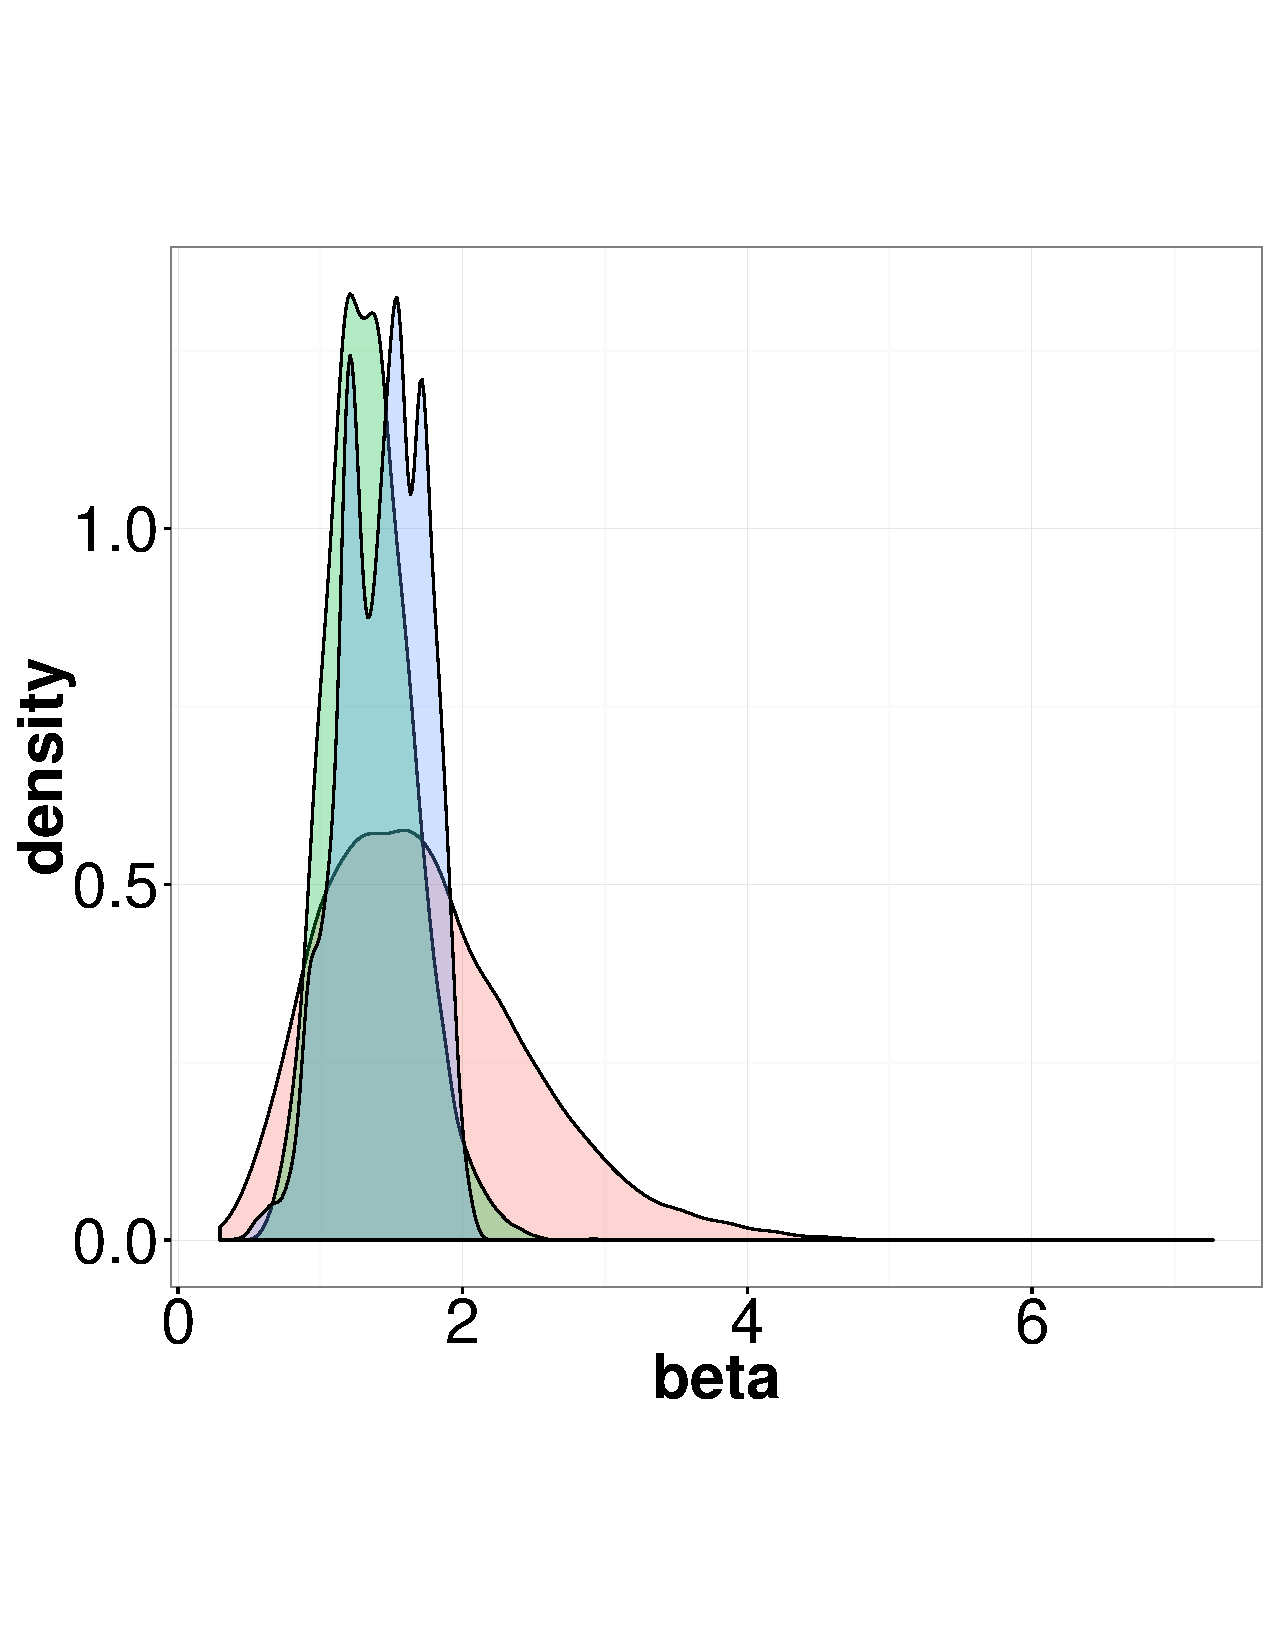
\includegraphics [width=0.98\textwidth, angle=0]{figs/dist_beta.pdf}
   \vspace{0.06 in}
  \end{minipage}
  \begin{minipage}[!hp]{0.3\linewidth}
  \centering
    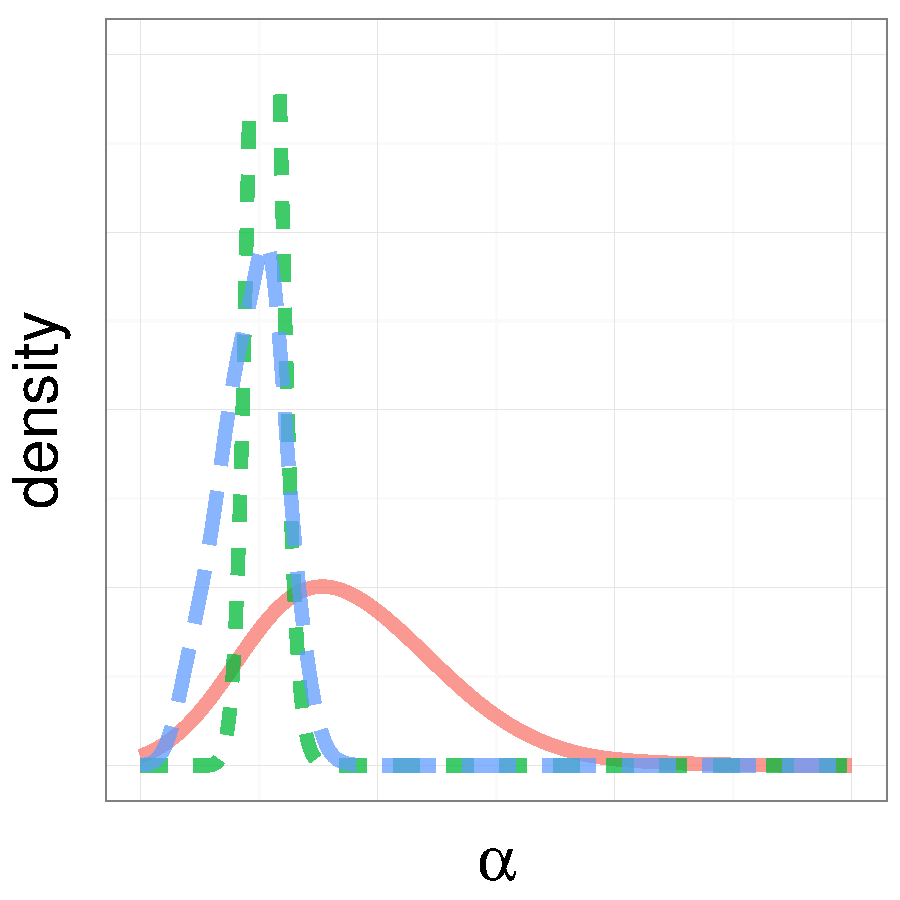
\includegraphics [width=0.98\textwidth, angle=0]{figs/dist_beta_100.pdf}
    \vspace{-0 in}
  \end{minipage}
  \vspace{-.3in}
  \caption{Prior density over an MJP parameter (solid curve), along with two conditionals: given observations only (long-dashes), and given observations and MJP path (short-dashes). 
    As $t_{end}$ increases from $10$ (left) to $100$ (right), the conditionals become more concentrated, implying strong path-parameter coupling. 
  The plots are from section~\ref{sec:immig}.}
     \label{fig:hist}
  \end{figure}
  However, the resulting Gibbs sampler can mix very poorly because of coupling between path and parameters.
  We illustrate this in figure~\ref{fig:hist}~\citep[inspired by][]{papaspiliopoulos2007general}), which shows the posterior distribution of an MJP parameter (long-dashes) is less concentrated than the distribution conditioned on both observations as well as path (short-dashes). 
  The coupling is strengthened as the trajectory grows longer (right panel), and the Gibbs sampler can mix very poorly with long observation periods, even if the observations themselves are only mildly informative about the parameters.

% \subsection{A marginal sampler for MJP parameters} 
% For the discrete-time case, this problem of parameter-trajectory
% coupling can be circumvented by marginalizing out the MJP trajectory 
% and directly sampling from the posterior over parameters $P(\theta|X)$.
% In its simplest form (Algorithm~\ref{alg:disc_time_mh}), this 
% involves a Metropolis-Hastings scheme that proposes a new parameter 
% $\vartheta$ from some proposal distribution 
% $q(\vartheta|\theta)$, accepting or rejecting according to the usual
% Metropolis-Hastings probability. The latter step requires calculating the 
% marginal probabilities $P(X|\theta)$ and $P(X|\theta')$, integrating out
% the exponential number of possible latent trajectories. Fortunately,
% this marginal probability is a by-product of the forward-backward
% algorithm used to sample a new trajectory, so that no 
% additional computational burden is involved. 
% %The overall algorithm then is:
% \begin{algorithm}[H]
%   \caption{Metropolis-Hastings parameter inference for a discrete-time 
% Markov chain}
%    \label{alg:disc_time_mh}
%   \begin{tabular}{l l}
%    \textbf{Input:  } & \text{Observations $X$},
%    proposal density $q(\vartheta|\ctheta)$, and 
%    \text{previous parameters $\ctheta$}.\\
%    \textbf{Output:  }& \text{A new Markov chain parameter $\ntheta$}.\\
%    \hline
%    \end{tabular}
%    \begin{algorithmic}[1]
%   \State Propose a new parameter $\vartheta$ from the proposal distribution
%   $q(\vartheta|\ctheta)$.
%   \State Run the forward pass of the forward-backward algorithm to 
%     obtain the marginal likelihood of the observations, $P(X|\vartheta)$.
%     \State Set $\ntheta = \vartheta$ with probability 
%     $\min(1,\frac{P(X,\vartheta)q(\ctheta|\vartheta)}{P(X,\ctheta)q(\vartheta|\ctheta)})$, else 
%     $\ntheta = \ctheta$.
%   \State Sample a new path with
%     the backward pass of the forward-backward algorithm.
%     %for the chosen parameter.
% \end{algorithmic}
% \end{algorithm}

% %\vspace{-.35in}
% Constructing a marginal sampler over the MJP parameters by
% integrating out the continuous-time trajectory is harder.
% %the set of transition times is unbounded, with individual elements
% %unconstrained over the observation interval $[0,\cT]$.
% %Naively calculating this marginal probability for the continuous-time
% %case is not straightforward, as there is no finite set of candidate
% %times to make a pass over. 
% One approach~\citep{FearnSher2006} makes a sequential 
% forward pass through all {\em observations} $X$, using matrix exponentiation
% to marginalize out all
% continuous-time paths between successive times. As
% shown in~\cite{RaoTeh13}, this approach is cubic rather than 
% quadratic in the 
% number of states, cannot exploit structure like sparsity in the 
% transition matrix, and can depend in not trivial ways on the exact 
% nature of the observation process.
% Also, the number of expensive matrix exponentiations depends on
% the number of observations rather than the number of transitions.
% %
% %
% A second approach, particle MCMC~\citep{Andrieu10}, uses 
% particle filtering to get an unbiased estimate of the marginal 
% $P(X|\theta)$. Plugging this into the Metropolis-Hastings 
% acceptance probability results in an MCMC sampler that targets the 
% correct posterior, however %~\cite{Andrieu09}, 
% the resulting scheme does not exploit the structure 
% of the MJP, and we show that it is quite inefficient.

% The advantage of introducing the thinned events $U$ was demonstrated in 
% \cite{RaoTeh13, RaoTeh12} : this allows exploiting discrete-time 
% algorithms like FFBS for path sampling.
% %be brought to playthe thinning-based approach over matrix exponential and particle-MCMC
% %approaches for trajectory inference. 
% In the next section, we outline a \naive\  first attempt at extending this 
% approach to 
% parameter inference.
% We describe why this approach is not adequate, and then describe our
% final algorithm. % in the section after. 
